\begin{figure}[tb]
\centering
% Auto-generated by make_rq3_figures.py -- do not edit manually.
% Required LaTeX setup (in the main document):
%   \usepackage{pgfplots}
%   \pgfplotsset{compat=1.18}
%   \usepgfplotslibrary{groupplots}  % only for the group figure

\definecolor{cf0}{RGB}{0,114,178}
\definecolor{cf1}{RGB}{213,94,0}
\definecolor{cf2}{RGB}{0,158,115}
\definecolor{cf3}{RGB}{230,159,0}
\definecolor{cf4}{RGB}{204,121,167}
\definecolor{cf5}{RGB}{86,180,233}

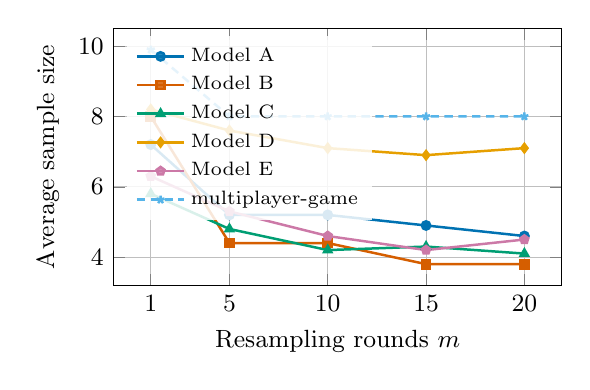
\begin{tikzpicture}
\begin{axis}[
width=0.6\textwidth,
height=0.4\textwidth,
title={},
xlabel={Resampling rounds $m$},
ylabel={Average sample size},
xtick={1,5,10,15,20},
grid=major,
tick label style={font=\small},
label style={font=\small},
title style={font=\small},
scaled y ticks=false,
yticklabel style={/pgf/number format/fixed},
legend pos=north west,
legend style={font=\scriptsize, draw=none, fill=white, fill opacity=0.85, text opacity=1},
legend cell align=left
]
\addplot+[color=cf0, mark=*, mark size=1.5pt, line width=0.9pt, mark options={solid}] coordinates { (1,7.2) (5,5.2) (10,5.2) (15,4.9) (20,4.6) };
\addlegendentry{Model A}
\addplot+[color=cf1, mark=square*, mark size=1.5pt, line width=0.9pt, mark options={solid}] coordinates { (1,8) (5,4.4) (10,4.4) (15,3.8) (20,3.8) };
\addlegendentry{Model B}
\addplot+[color=cf2, mark=triangle*, mark size=1.5pt, line width=0.9pt, mark options={solid}] coordinates { (1,5.8) (5,4.8) (10,4.2) (15,4.3) (20,4.1) };
\addlegendentry{Model C}
\addplot+[color=cf3, mark=diamond*, mark size=1.5pt, line width=0.9pt, mark options={solid}] coordinates { (1,8.2) (5,7.6) (10,7.1) (15,6.9) (20,7.1) };
\addlegendentry{Model D}
\addplot+[color=cf4, mark=pentagon*, mark size=1.5pt, line width=0.9pt, mark options={solid}] coordinates { (1,6.3) (5,5.3) (10,4.6) (15,4.2) (20,4.5) };
\addlegendentry{Model E}
\addplot+[color=cf5, mark=star, mark size=1.5pt, line width=0.9pt, mark options={solid}] coordinates { (1,9.9) (5,8) (10,8) (15,8) (20,8) };
\addlegendentry{multiplayer-game}
\end{axis}
\end{tikzpicture}

\caption{Influence of the number of resampling rounds $m$ on the sample size of the instance-set $t$-wise sampling algorithm. Lines show the evaluation models; averages over $r=10$ repetitions ($r=5$ for Model B) with $t=2$ and $c=50$.}
\label{fig:rq3-size}
\end{figure}
